\documentclass[a4paper,12pt]{article}
\usepackage[DIV=14,BCOR=0mm,headinclude=true,footinclude=false]{typearea}
\usepackage{graphicx}
\usepackage[bottom]{footmisc}
\usepackage[titletoc]{appendix}
\usepackage{hyperref}
\usepackage{listings}
\usepackage{float}
\usepackage{amsmath}
\usepackage{mathrsfs}
\usepackage{amssymb}
\usepackage{braket}

\newcommand{\code}[1]{\texttt{#1}}
\def\be{\begin{equation}}
\def\ee{\end{equation}}
\def\ba{\begin{aligned}}
\def\ea{\end{aligned}}
\title{PHYS-GA-2000 Computational Physics \\ FINAL PROJECT \\ Simulating the Penrose Process }
\author{Panagiotis Charalambous}


\begin{document}

\maketitle

\begin{abstract}
	We have written a \code{python} program solving geodesics with only inputs the coordinate system used along with the metric tensor components in that particular coordinate basis and non-gravitational forces. After demonstrating the code's correctness, we use it to simulate the Penrose process,observable in rotating black holes.
\end{abstract}

\tableofcontents
\listoffigures
\listoftables

\section{Introduction}
\label{Sec1}

We aim to investigate the geodesic equations for the motion of a massive particle in the presence of a background gravitational field. The dimensionality of the spacetime itself is left as an input parameter along with the metric tensor. For a formal introduction to General Relativity, we recommend the reader to be advised from \cite{WeinbergGR} or \cite{GR_Carroll}.

The geodesic equations are in general,
\be
	\ddot{x}^{\rho} + \Gamma^{\rho}_{\mu\nu}\dot{x}^{\mu}\dot{x}^{\nu} = 0
\ee
where, ``dots'' represent derivatives with respect to the affine parameter $\lambda$, e.g. $\dot{x}^{\mu} \equiv \frac{dx^{\mu}}{d\lambda}$, and $\Gamma^{\rho}_{\mu\nu}$ are the Christoffel symbols whose components in a coordinate basis are obtained by first derivatives of the metric tensor,
\be\label{Christoffel}
	\Gamma^{\rho}_{\mu\nu} = \frac{1}{2}g^{\rho\sigma}\left( \partial_{\mu}g_{\sigma\nu} + \partial_{\nu}g_{\mu\sigma} - \partial_{\sigma}g_{\mu\nu} \right)
\ee

The geodesic equations in ($D=d+1$)-dimensions are a set of $D$ coupled second-order ordinary differential equations and can equivalently be written as $2D$ coupled first-order ordinary differential equations by introducing the $D$-velocities, $u^{\mu} \equiv \dot{x}^{\mu}$, allowing to write our problem as,
\be\ba
	\dot{x}^{\rho} &= u^{\rho} \;\;\;\;\;\;\;\;\;\;\;\;\;\;\;\;\;\;\,:\;\; D\text{ equations} \\
	\dot{u}^{\rho} &= -\Gamma^{\rho}_{\mu\nu}(x)u^{\mu}u^{\nu} \;\;:\;\; D\text{ equations}
\ea\ee

We are more interested to see how the massive particle propagates according to a stationary observer, that is, we set the affine parameter to the proper time $\tau$ and measure time using the coordinate time $x^0\equiv t$ by also introducing the coordinate velocity, $\upsilon^{\mu} \equiv \frac{dx^{\mu}}{dt} = (1,\vec{\upsilon})$. In terms of these, the equations of motion read (Appendix \ref{ApA}),
\be\ba\label{EOM}
	\frac{dx^{i}}{dt} &= \upsilon^{i} \\
	\frac{d\upsilon^{i}}{dt} &= -\Gamma^{i}_{00} + \left(\Gamma^{0}_{00}\delta^{i}_{j} - 2\Gamma^{i}_{0j}\right)\upsilon^{j} + \left(2\Gamma^{0}_{0j}\delta^{i}_{k} - \Gamma^{i}_{jk}\right)\upsilon^{j}\upsilon^{k} + \Gamma^{0}_{jk}\upsilon^{i}\upsilon^{j}\upsilon^{k}
\ea\ee

If there are additional, non-gravitational, forces, e.g. electromagnetic interaction of a charged particle with a charged black hole, then the $D$-acceleration $a^{\mu}$ associated with non-gravitational interactions adds a new term in the equations of motion. The geodesics become,
\be
	\ddot{x}^{\rho} + \Gamma^{\rho}_{\mu\nu}\dot{x}^{\mu}\dot{x}^{\nu} = a^{\rho}
\ee
and the subsequent coordinate equations of motion turn out to be,
\be\ba\label{EOM_F}
	\frac{dx^{i}}{dt} &= \upsilon^{i} \\
	\frac{d\upsilon^{i}}{dt} &= -\bigg(\Gamma^{i}_{00} + a^{i}g_{00} \bigg) + \bigg(\left(\Gamma^{0}_{00} + a^{0} \right) \delta^{i}_{j} - 2\left(\Gamma^{i}_{0j}+a^{i}g_{0j}\right)\bigg)\upsilon^{j} + \\
	&+ \bigg(2\left(\Gamma^{0}_{0j}+a^{0}g_{0j}\right)\delta^{i}_{k} - \left(\Gamma^{i}_{jk} + a^{i}g_{jk}\right)\bigg)\upsilon^{j}\upsilon^{k} + \bigg(\Gamma^{0}_{jk}+a^{0}g_{jk}\bigg)\upsilon^{i}\upsilon^{j}\upsilon^{k}
\ea\ee
We treat the extra $D$-acceleration $a^{\mu}$ as an additional input. We leave as a future development to take as an input the interaction Lagrangian rather than the $D$-acceleration (see Appendix \ref{ApC}). This would allow to directly construct both the $D$-acceleration $a^{\mu}$ \textit{and} the conjugate momenta $P^{\mu}$ associated with useful observables such as the energy and the angular momentum of the particle.
\section{Part A: Soling Geodesics}
\label{Sec2}

Using the python library \code{sympy}\footnote{This does not come directly by installing python using the \code{pip} command. To install it, simply type, \code{pip install --user sympy}.}, we evaluate the Christoffel symbols \eqref{Christoffel} and then use them to construct the force functions on the right-hand side of \eqref{EOM} for the coordinate velocities by also inputting the additional $D$-acceleration $a^{\mu}$.

We have implemented different integration schemes seen in class. Namely, we have implemented Forward Euler, RK2, RK4, Leapfrog and Verlet as well as the adaptive step size versions for the explicit integrators.
%The five integration schemes have the following difference equations,
% WRITE DIFFERENCE EQUATIONS FOR 5 INTEGRATORS

The inputs and outputs of the program are as the following tables \ref{tbl:INPUT} and \ref{tbl:OUTPUT} indicate respectively,
\begin{table}[H]
	\centering
	\begin{tabular}{|c|c|}
		\hline
		Input Parameters & Description \\
		\hline
		\hline
		$x^{\mu}$ & Coordinate system to be used \\
		\hline
		$g_{\mu\nu}(x)$ & Metric tensor components in the $\{x^{\mu}\}$-coordinate system \\
		\hline
		$a^{\mu}$ & $D$-acceleration associated with non-gravitational interaction \\
		\hline
		$t_0$ & Initial coordinate time instant \\
		\hline
		$t_{N}$ & Final coordinate time instant \\
		\hline
		$N$ & Number of time steps to be taken \\
		\hline
		$x^{i}_0$, $i=1,\dots,D-1$ & Initial spatial position at coordinate time $t_0$\\
		\hline
		$\upsilon^{i}_0$, $i=1,\dots,D-1$ & Initial coordinate spatial velocity at coordinate time $t_0$\\
		\hline
		INTEGRATOR & Integration scheme to be used \\
		\hline
	\end{tabular}
	\caption{Input parameters}
	\label{tbl:INPUT}
\end{table}

\begin{table}[H]
	\centering
	\begin{tabular}{|c|c|}
		\hline
		Output Parameters & Description \\
		\hline
		\hline
		$x^{i}(t)$, $i=1,\dots,D-1$ & Spatial position at coordinates times $t\in[t_{0},t_{N}]$ \\
		\hline
		$\upsilon^{i}(t)$, $i=1,\dots,D-1$ & Spatial coordinate velocity at coordinate times $t\in[t_{0},t_{N}]$\\
		\hline
		$u_{\mu}(t)$, $i=0,\dots,D-1$ & Covariant $D$-velocity at coordinate times $t\in[t_{0},t_{N}]$\\
		\hline
	\end{tabular}
	\caption{Output parameters}
	\label{tbl:OUTPUT}
\end{table}

From the covariant $D$-velocity, one can also read the energy and angular momentum of the particle around the $x_{D-1}$-axes whose rotations are associated with the azimuthal angle $\phi \equiv \theta_{D-1}$ when using spherical coordinates,
\be\ba
	E &\equiv -mu_{0} \\
	L &\equiv mu_{D-1}
\ea\ee

\subsection{Schwarzschild Metric}
As a first test, we solve the geodesics for motion around a Schwarzschild black hole whose geometry is,
\be\ba
	ds_{S}^2 &= -f_{S}(r)dt^2 + \frac{dr^2}{f_{S}(r)} + r^2d\Omega_{D-2}^2 \\
	f_{S}(r) &= 1-\left(\frac{R_{S}}{r}\right)^{D-3}
\ea\ee
where $R_{S}$ is the Schwarzschild radius related to the mass $M$ of the black hole (ADM mass) according to,
\be
	R_{S}^{D-3} = \frac{16\pi GM}{(D-2)\Omega_{D-2}}
\ee
with $\Omega_{D-2}$ the surface of a unit $(D-1)$-dimensional sphere,
\be
	\Omega_{D-2} = Area(S^{D-2}) = (D-1)\frac{\pi^{\frac{D-1}{2}}}{\Gamma\left(\frac{D+1}{2}\right)}
\ee
and $d\Omega_{D-2}^2$ is the infinitesimal length on $S^{D-2}$,
\be
	d\Omega_{D-2}^{2} = \sum_{n=2}^{D-1}\left(\prod_{m=2}^{n-1}\sin^2\theta_{m}\right)d\theta_{n}^2
\ee
Note that we have indexed the angle variables from $2$ to $D-1$ to remind that the $x^1$ coordinate is $r$.

The Schwarzschild black hole is equipped with an event horizon\footnote{The event horizons are null surfaces. For the case of the event horizons located at the surfaces of constant radial coordinate $r_{H} = const.$, the condition they must obey is $g^{rr}\mid_{r=r_{H}}=0$.} at precisely the Schwarzschild radius,
\be
	r_{H} = R_{S}
\ee
and signifies the limit of no return. Quite remarkably, a stationary observe will never see the massive particle falling inside the black hole; the particle will appear to slow down near the event horizon until it finally freezes at $r=r_{H}$ and disappears due to infinite redshift. This is a property of all black hole solutions.

\subsubsection{Run 1: Bound trajectory}
For the first run, we take $D=4$ and the following initial conditions,
\begin{table}[H]
	\centering
	\begin{tabular}{|c|c|}
		\hline
		$t_0$ & 0.0 \\
		\hline
		$r_0$ & 10.0 \\
		\hline
		$\theta_0$ & $\frac{\pi}{2}$ \\
		\hline
		$\phi_0$ & 0.0 \\
		\hline
		\hline
		$\upsilon_{r0}$ & -0.03 \\
		\hline
		$\upsilon_{\theta0}$ & 0.0 \\
		\hline
		$\upsilon_{\phi0}$ & 0.03 \\
		\hline
	\end{tabular}
	\caption[Run 1: Initial Conditions]{Run 1: Initial Conditions.}
	\label{tbl:RUN1_IC}
\end{table}

These initial conditions ensure a specific energy $\frac{E}{m} = 0.9501784 < 1$ allowing a bound trajectory. Running using the RK4 integrator with $N=10000$ iterations and final time instant $t_{N} = 1000.0$, we output figures \ref{fig:RUN1_xv} and \ref{fig:RUN1_U}.

\begin{figure}
	\centering
	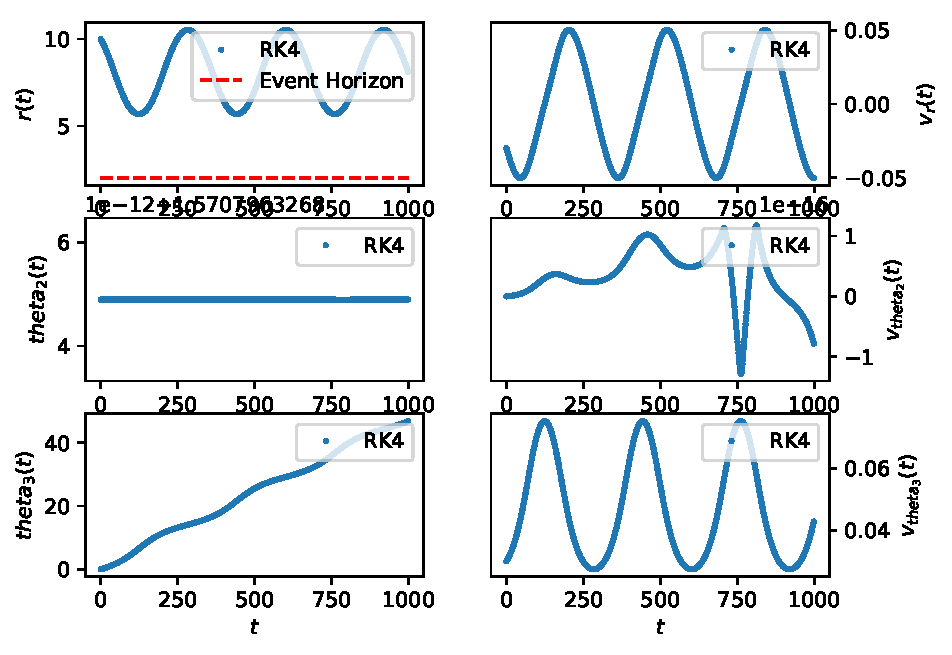
\includegraphics[height=8cm]{Figures/xv_t_Rotating.pdf}
	\caption[Run 1: Coordinate positions and velocities]{Run 1: Coordinate positions and velocities for a bound trajectory in 4-dimensional Schwarzschild solution.}
	\label{fig:RUN1_xv}
\end{figure}

\begin{figure}
	\centering
	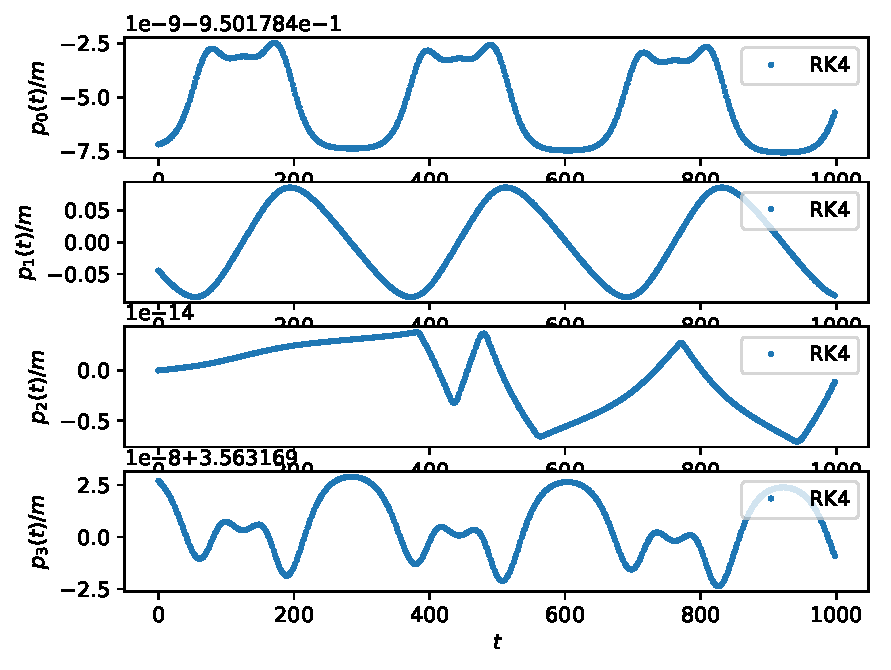
\includegraphics[height=8cm]{Figures/U_t_Rotating.pdf}
	\caption[Run 1: 4-velocity]{Run 1: 4-velocity components for a bound trajectory in 4-dimensional Schwarzschild solution.}
	\label{fig:RUN1_U}
\end{figure}

\subsubsection{Run 2: Doomed trajectory}
For the second run, we take $D=4$ and the following initial conditions,
\begin{table}[H]
	\centering
	\begin{tabular}{|c|c|}
		\hline
		$t_0$ & 0.0 \\
		\hline
		$r_0$ & 3.0 \\
		\hline
		$\theta_0$ & $\frac{\pi}{2}$ \\
		\hline
		$\phi_0$ & 0.0 \\
		\hline
		\hline
		$\upsilon_{r0}$ & -0.3 \\
		\hline
		$\upsilon_{\theta0}$ & 0.0 \\
		\hline
		$\upsilon_{\phi0}$ & 0.0 \\
		\hline
	\end{tabular}
	\caption[Run 2: Initial Conditions]{Run 2: Initial Conditions.}
	\label{tbl:RUN2_IC}
\end{table}

These initial conditions account for an unbound trajectory with a specific energy $\frac{E}{m} = 1.41833 > 1$ but the angular velocity $\upsilon_{\phi0}$ is small enough to not escape the black hole. Running using the RK4 integrator again with $N=300$ steps and final time instant $t_{N} = 10.0$, we output figures \ref{fig:RUN2_xv} and \ref{fig:RUN2_U}.

\begin{figure}
	\centering
	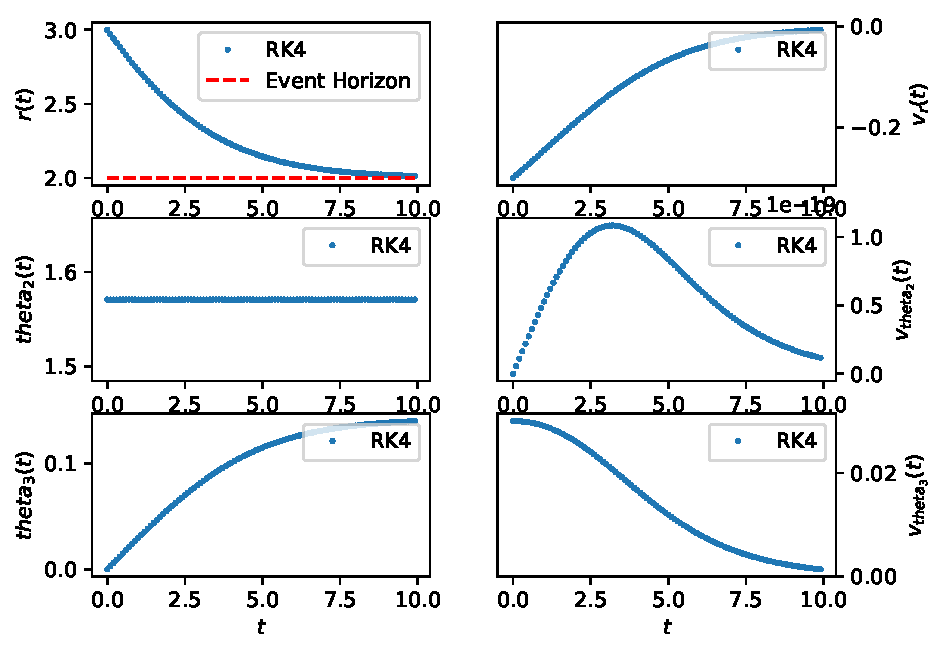
\includegraphics[height=8cm]{Figures/xv_t_Falling.pdf}
	\caption[Run 2: Coordinate positions and velocities]{Run 2: Coordinate positions and velocities for an unbound, doomed trajectory in 4-dimensional Schwarzschild solution.}
	\label{fig:RUN2_xv}
\end{figure}

\begin{figure}
	\centering
	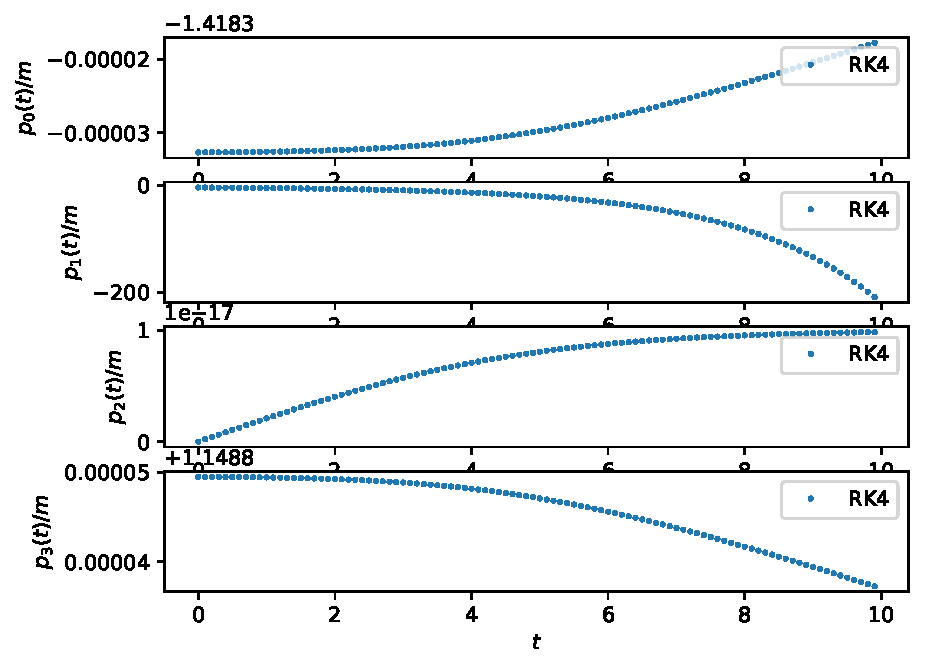
\includegraphics[height=8cm]{Figures/U_t_Falling.pdf}
	\caption[Run 2: 4-velocity]{Run 2: 4-velocity components for a unbound, doomed trajectory in 4-dimensional Schwarzschild solution.}
	\label{fig:RUN2_U}
\end{figure}

\subsection{Reissner-Nordstr\"{o}m Metric}
A second test, would be to run our program for motion around a Reissner-Nordstro\"{o}m black hole,
\be\ba
	ds_{RN}^2 &= -f_{RN}(r)dt^2 + \frac{dr^2}{f_{RN}(r)} + r^2d\Omega_{D-2}^2 \\
	f_{RN}(r) &= 1-\left(\frac{R_{S}}{r}\right)^{D-3} + \left(\frac{A}{r}\right)^{2(D-3)}
\ea\ee
where $A$ is related to the total charge $Q$ of the black hole according to,
\be
	A^{2(D-3)} = \frac{8\pi GQ^2}{(D-2)(D-3)}
\ee

In contrast to the Schwarzschild solution, the Reissner-Nordstr\"{o}m black hole has two event horizons,
\be
	r_{H}^{\pm} = \frac{R_{S}}{2}\left( 1 \pm \sqrt{1 - 4\left(\frac{A}{R_{S}}\right)^{2(D-3)}} \right)^{\frac{1}{D-3}}
\ee
from which, however, only the outer horizon can be formed from physical processes, $r_{H} = r_{H}^{+}$; the inner event horizon is a mathematical artifact.

This run would also test the implementation of additional non-gravitational forces. We leave this analysis for future development.
\section{Part B: Simulating the Penrose Process}
\label{Sec3}

\subsection{Kerr-Newman Metric}
For the final attempt, we are interested in the 4-dimensional rotating black hole and the investigation of the Penrose process. The metric of a 4-dimensional axisymmetric, stationary black hole in asymptotically flat spacetime is given by the Kerr-Newman solution,
\be\ba\label{Metric_Kerr-Newman}
	ds^2 = &-\frac{\Delta - a^2\sin^2\theta}{\Sigma}dt^2 + \frac{\Sigma}{\Delta}dr^2 + \Sigma d\theta^2 + \\
	&+ \frac{\left(r^2+a^2\right)^2 - a^2\Delta\sin^2\theta}{\Sigma}\sin^2\theta d\phi^2 - 2\frac{R_{S}ra\sin^2\theta}{\Sigma}dtd\phi
\ea\ee
with,
\be\ba
	\Delta &= r^2 + a^2 - R_{S}r + Q^2 \\
	\Sigma &= r^2 + a^2\cos^2\theta
\ea\ee
The parameters $R_{S}$, $a$ and $Q$ are the Schwarzschild radius, $R_{S}=2GM$, the spin parameter, $a=\frac{J}{M}$, with $J$ the angular momentum of the black hole around the $z$-axes, and the electric charge of the black hole respectively. This solution also has two event horizons,
\be
	r_{H}^{\pm} = \frac{R_{S}}{2}\left( 1 \pm \sqrt{1 - 4\frac{a^2 + Q^2}{R_{S}^2}} \right)
\ee
with only the outer horizon being physical, $r_{H} = r_{H}^{+}$.

Apart from the event horizons, the rotating black hole possesses a unique region, called the ergoregion. This is the region within which a particle cannot stay still and is given by the set of those points satisfying $g_{tt}>0$. As a result. The ergoregion is bounded by two ergospheres $r_{E}^{\pm}$ ( $r_{E}^{-} < r < r_{E}^{+}$),
\be
	r_{E}^{\pm} = \frac{R_{S}}{2}\left( 1 \pm \sqrt{1 - 4\frac{a^2\cos^2\theta + Q^2}{R_{S}^2}}  \right)
\ee
but only $r_{E}^{+} \equiv r_{E}$ is physical, while $r_{E}^{-} < r_{H}^{-}$ so, the real ergoregion is $r_{H}<r<r_{E}$.

\subsection{Penrose Process}
In 1971, Roger Penrose and R. M. Floyd (\cite{Penrose1971}) theorized the extraction of energy from a rotating black hole through a simple mechanism. The procedure is as in figure \ref{fig:PenroseProcess}. A parent particle (particle 1) with some energy $E_1$ decays into an outgoing particle (particle 2) with energy $E_2$ and an ingoing particle (particle 3) with energy $E_3$. Under special conditions, $E_3$ can be negative allowing particle 2 to be detected by a distant observer with an increased energy.

The condition for a negative energy is a $\phi$-component of the coordinate velocity smaller than a critical value,
\be\label{NES_vd}
	\upsilon^{\phi} < -\frac{g_{tt}}{g_{t\phi}} < 0
\ee
This also sets an allowed range of the specific angular momentum $l\equiv\frac{L}{m}$,
\be\label{NES_l}
	l < -\sqrt{\frac{-\psi g_{\phi\phi}}{g_{t\phi}^2g_{tt}}}
\ee
where $\psi = g_{tt}g_{t\phi} - g_{t\phi}^2 = -\Delta\sin^2\theta <0 $ is the determinant of the sub-metric $2\times2$ matrix constructed only from $t$ and $\phi$ components,
\be
	\tilde{g} = \begin{pmatrix}
		g_{tt} & g_{t\phi} \\
		g_{\phi t} & g_{\phi\phi}
	\end{pmatrix}
	\Rightarrow \tilde{g}^{-1} = \frac{1}{\psi} \begin{pmatrix}
		g_{\phi\phi} & -g_{t\phi} \\
		-g_{\phi t} & g_{tt}
	\end{pmatrix}
\ee
From the specific angular momentum condition \eqref{NES_l}, it is obvious that the Penrose process can be produced only when $g_{tt}<0$, i.e. only within the ergoregion. The negative sign in \eqref{NES_l} also shows that the particle must have an opposite angular momentum ($L<0$) from the angular momentum of the black hole ($J>0$). Evidentially, a careful analysis of the process reveals that the extra energy particle 2 has gained comes from the rotational energy of the black hole; particle 3 is absorbed by the black hole lowering its total angular momentum to $J^{\prime} = J + L<J$.

\begin{figure}
	\centering
	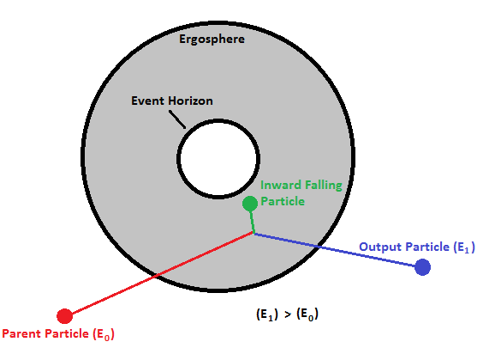
\includegraphics[height=8cm]{Figures/PenroseProcess.png}
	\caption[Mechanical Penrose Process]{Mechanical Penrose Process. A parent particle falls from infinity towards the black hole and decays into a new ingoing particle and an outgoing particle. The second in-falling particle can have negative energy within the ergoregion allowing the outgoing particle to be detected with increased energy from a distant observer.}
	\label{fig:PenroseProcess}
\end{figure}

At the point of split, conservation of 4-momentum must be satisfied,
\be
	p_{1\mu} = p_{2\mu} + p_{3\mu}
\ee
To simplify the problem, we consider equatorial motion, that is, we set $\theta = \frac{\pi}{2}$ and $\upsilon_1^{\theta} = \upsilon_2^{\theta} =\upsilon_3^{\theta} = 0$\footnote{It is simple to prove that, if the initial $\theta$-component of the coordinate velocity is zero at the equatorial plane, then it stays zero along the entire propagation. This follows from the conservation of the angular momentum $L$ which ensures that the motion is restricted to the plane perpendicular to $\vec{L} = L\hat{z}$}. In addition, to further simplify the simulation, we take $\upsilon_3^{r} = 0$. As a result, conservation of 4-momentum is expanded to the following 3 constraints,
\be\label{E_CONS}
	\epsilon_1 = \mu_2 \epsilon_2 + \mu_3 \epsilon_3 \Rightarrow \boxed{\epsilon_2 = \frac{\epsilon_1 - \mu_3 \epsilon_3}{\mu_2}}
\ee
\be\label{ur_CONS}
	\dot{t}_1 \upsilon_{1}^{r} = \mu_2 \dot{t}_2 \upsilon_{2}^{r} \Rightarrow \boxed{\upsilon_{2}^{r} = -\frac{\dot{t}_1\upsilon_{1}^{r}}{\mu_2}}
\ee
\be\label{L_CONS}
	l_1 = \mu_2 l_2 + \mu_3 l_3 \Rightarrow \boxed{l_{2} = \frac{l_1 - \mu_3 l_3}{\mu_2}}
\ee
where $\epsilon\equiv\frac{E}{m}$ and $l\equiv\frac{L}{m}$ are the specific energy and specific angular momentum respectively and $\mu_2$ and $\mu_3$ are the ratios of the masses of particles 2 and 3 over the mass of the parent particle, $\mu_2 \equiv \frac{m_2}{m_1}$, $\mu_3\equiv\frac{m_3}{m_1}$. In addition, we have a constraint following from $p^2 = -m^2$,
\be\label{M_CONS}
	p_2^2 = (p_1 - p_3)^2 = p_1^2 + p_3^2 - 2p_{1} \cdot p_{3} \Rightarrow \boxed{\mu_2 = \sqrt{1+\mu_3^2 + 2\mu_3 u_1 \cdot u_{3}}}
\ee

From these 4 equations, we can solve for $\upsilon_{2}^{r}$, $\upsilon_{2}^{\phi}$, $\mu_2$ and $\mu_3$ given the $\phi$-component of the coordinate velocity $\upsilon_{3}^{\phi}$ of particle 3. This is chosen to ensure that it has negative energy, that is, we take the splitting to take place within the ergoregion $r_{H}<r<r_{E}$ and $\upsilon_{3}^{\phi} < -\frac{g_{tt}}{g_{t\phi}}$.

To sum up so far, the known quantities are $\vec{\upsilon}_1 = (\upsilon_{1}^{r},0,\upsilon_{1}^{\phi})$ and $\vec{\upsilon}_3 = (0,0,\upsilon_{3}^{\phi})$, while the unknown quantities are $\vec{\upsilon}_2 = (\upsilon_{2}^{r},0,\upsilon_{2}^{\phi})$, $\mu_2$ and $\mu_3$.

Solving \eqref{ur_CONS}, we find that,
\be\label{v2r}
	\upsilon_{2}^{r} = \sqrt{-\frac{\lambda_1^2}{\lambda_1^2 g_{rr} + \mu_2^2}\left( g_{tt}+2g_{t\phi}\upsilon_{2}^{\phi} + g_{\phi\phi}(\upsilon_{2}^{\phi})^2 \right)}
\ee
where $\lambda_1 \equiv \dot{t}_1\upsilon_{1}^{r}$. We have chosen the ``$+$'' sign to ensure that particle heads out and is not in danger of getting too close to the event horizon before escaping to infinity. Plugging this expression into the expression of $l_2 \equiv u_{2\phi}$ and using \eqref{L_CONS}, we find that,
\be
	\upsilon_{2}^{\phi} = g_{tt} \frac{-g_{t\phi} + \sqrt{-\psi}\sqrt{k(k+1)}}{g_{t\phi}^2 + kg_{tt}g_{\phi\phi}}
\ee
where the parameter $k$ is given by,
\be
	k = \left(\frac{\mu_3 l_3}{\mu_2}\right)^2\left(1-\frac{\lambda_1^2}{\lambda_1^2g_{rr}+\mu_2^2}\right)
\ee
Finally, use this result of $\upsilon_{2}^{\phi}$ to also write $\upsilon_{2}^{r}$ in terms of $\mu_2$ and $\mu_3$ and use \eqref{E_CONS} and \eqref{M_CONS} to solve for $\mu_2$ and $\mu_3$. This could in principle be done analytically but the calculations are too much so we instead be lazy and solve the system computationally using the Newton-Raphson method.

\subsection{Constraints on $\mu_2$ and $\mu_3$}
We can see that $\upsilon_{2}^{r}>0$ always exists\footnote{One could argue that $g_{tt}+2g_{t\phi}\upsilon_1^{\phi}+g_{\phi\phi}(\upsilon_{1}^{\phi})^2$ must be negative, but this follows directly from the fact that the particles are massive. This means that,
	\be\ba
		&-\dot{t}^{-2} = g_{tt} + 2g_{t\phi} + g_{rr}(\upsilon^{r})^2 + g_{\phi\phi}(\upsilon^{\phi})^2 < 0 \\
		&\Rightarrow g_{tt} + 2g_{t\phi} + g_{\phi\phi}(\upsilon^{\phi})^2 < -g_{rr}(\upsilon^{r})^2 < 0
	\ea\ee
given that the particle is outside the black hole ($r>r_{H}\Rightarrow g_{rr}>0$).}. The existence of $\upsilon_{2}^{\phi}$, however, requires that,
\be
	k(k+1) \ge 0 \Rightarrow k\ge0 \;\; or \;\; k\le-1
\ee
The first case of $k\ge0$ is always satisfied unless $g_{rr}\le1$ but that would require the particle to be inside the black hole\footnote{Expanding $g_{rr}\le1$ from \eqref{Metric_Kerr-Newman}, we find that $r\le\frac{a^2+Q^2}{R_{S}}$. Physical black holes are not naked singularities, meaning that the event horizon exists, i.e. $\frac{a^2+Q^2}{R_{S}}\le\frac{R_{S}}{4}$. Consequently, if $g_{rr}\le1$, then $r\le\frac{R_{S}}{4}$ but $\frac{R_{S}}{4}<r_{H}$.}. On the other hand, $k\le-1$ can never be achieved because it yields the condition,
\be
	\mu_3^2 \le \frac{\mu_2^2}{-g_{tt}l_3^2} \frac{\lambda_1^2g_{rr} + \mu_2^2}{\lambda_1^2(1-g_{rr}) - \mu_2^2} < 0
\ee

The only true constraint on $\mu_2$ and $\mu_3$ is the requirement of particle 2 to reach infinity. This requires $\epsilon_2\ge1$ so,
\be
	\boxed{\mu_2 \le \epsilon_1 - \mu_3 \epsilon_3}
\ee

A natural process will also have $\mu_2^2 + \mu_3^2 < 1$ because,
\be
	p_1^2 = p_2^2 + p_3^2 + 2p_2 \cdot p_3 \Rightarrow \mu_2^2 + \mu_3^2 = 1 + 2p_2 \cdot p_3 < 1
\ee
since particles 2 and 3 are timelike-separated, i.e. $p_2 \cdot p_3 < 0$.

\subsection{Run 3: Results}
The rotating black hole we simulated has $J=0.9$ and $Q=0.0$. We firstly solved the geodesics using part A to simulate the propagation of the parent particle from very far $r = 100R_{S} = 200.0$ until somewhere near the black hole $r \sim r_{H} $. Then we used those values of $\{t,\vec{x},\vec{v}\}$ for the parent particle at $r\sim6.0$ as initial conditions to simulate the process. We propagated the parent particle until $r_{H} < r < r_{E}$ and then perform the splitting into particles 2 and 3 according to the above discussion.

The initial conditions for the parent particle were,
\begin{table}[H]
	\centering
	\begin{tabular}{|c|c|}
		\hline
		$t_{10}$ & 3176.535 \\
		\hline
		$r_{10}$ & 6.103719 \\
		\hline
		$\theta_{10}$ & $\frac{\pi}{2}$ \\
		\hline
		$\phi_{10}$ & 0.072048 \\
		\hline
		\hline
		$\upsilon_{1r0}$ & -0.386224 \\
		\hline
		$\upsilon_{1\theta0}$ & 0.0 \\
		\hline
		$\upsilon_{1\phi0}$ & 0.00769361 \\
		\hline
	\end{tabular}
	\caption[Run 3: Initial Conditions for parent particle]{Run 3: Initial Conditions for parent particle.}
	\label{tbl:RUN3_IC}
\end{table}

We set the final time instant to $t_{N}=3191.4575$ for which the final position for particle 1 and initial positions for particles 2 and 3 are,
\begin{table}[H]
	\centering
	\begin{tabular}{|c|c|}
		\hline
		$t_{02,3}$ & 3191.4425775 \\
		\hline
		$r_{02,3}$ & 1.72223189 \\
		\hline
		$\theta_{02,3}$ & $\frac{\pi}{2}$ \\
		\hline
		$\phi_{02,3}$ & 1.15216234 \\
		\hline
	\end{tabular}
	\caption[Run 3: Initial positions for particles 2 and 3]{Run 3: Initial positions for particles 2 and 3.}
	\label{tbl:RUN3_IC2}
\end{table}
After solving the equations for $\mu_3$, $\mu_2$ and the initial velocity for particle 2, we arrive at the following results,
\begin{table}[H]
	\centering
	\begin{tabular}{|c|c|}
		\hline
		$v_{2r0}$ & 0.08684806 \\
		\hline
		$v_{2\theta0}$ & 0.0 \\
		\hline
		$v_{2\phi0}$ & 0.22415412 \\
		\hline
		\hline
		$v_{3r0}$ & 0.0 \\
		\hline
		$v_{3\theta0}$ & 0.0 \\
		\hline
		$v_{3\phi0}$ & 0.09949532 \\
		\hline
	\end{tabular}
	\caption[Run 3: Initial velocities for particles 2 and 3]{Run 3: Initial velocities for particles 2 and 3.}
	\label{tbl:RUN3_IC3}
\end{table}
\begin{table}[H]
	\centering
	\begin{tabular}{|c|c|}
		\hline
		$\mu_2$ & $0.738561712$ \\
		\hline
		$\mu_3$ & $1.47921968 \cdot 10^{-5}$ \\
		\hline
	\end{tabular}
	\caption[Run 3: Masses of particles 2 and 3]{Run 3: Masses of particles 2 and 3.}
	\label{tbl:RUN3_IC4}
\end{table}

The specific energies of particles 1,2 and 3 are then,
\begin{table}[H]
	\centering
	\begin{tabular}{|c|c|}
		\hline
		$\epsilon_1$ & $0.994987723$ \\
		\hline
		$\epsilon_2$ & $1.37619187$ \\
		\hline
		$\epsilon_3$ & $-1.447716 \cdot 10^{3}$ \\
		\hline
	\end{tabular}
	\caption[Run 3: Specific energies of particles 1, 2 and 3]{Run 3: Specific energies of particles 1, 2 and 3.}
	\label{tbl:RUN3_IC5}
\end{table}

Finally, we solved the geodesics for particles 2 and 3 separately with final time instants $t_{2N}=5000.0$, $t_{3N}=3206.442575$ and number of time steps $N_2 = N_3 = 15000$. The relevant graphs are figures %\ref{fig:RUN3_xv} and \ref{fig:RUN3_U}.

\begin{figure}
	\centering
	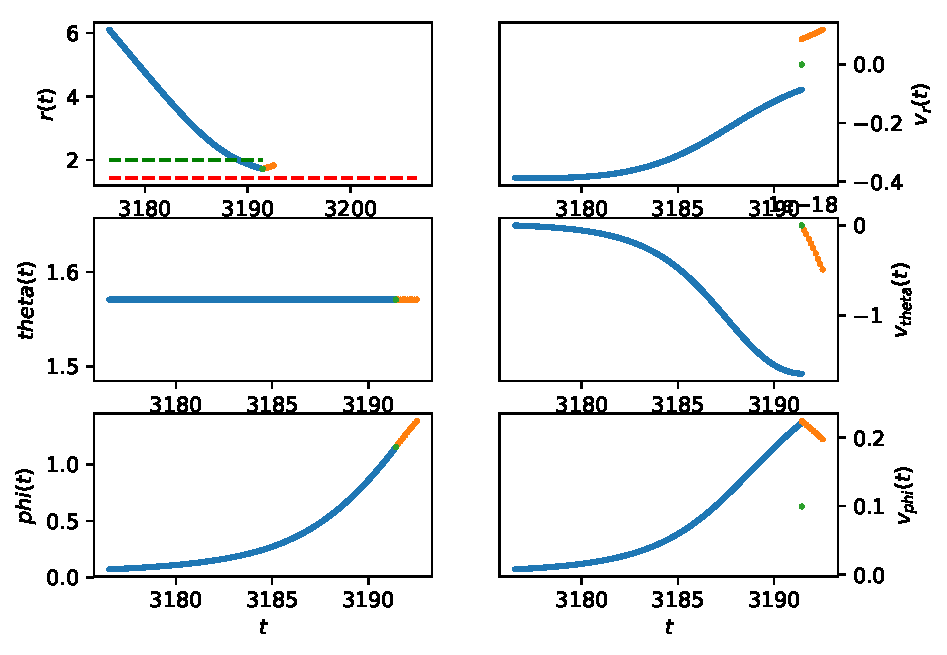
\includegraphics[height=8cm]{Figures/xv_t_Penrose.pdf}
	\caption[Run 3: Coordinate positions and velocities]{Run 3: Coordinate positions and velocities for the simulated Penrose process.}
	\label{fig:RUN3_xv}
\end{figure}

\begin{figure}
	\centering
	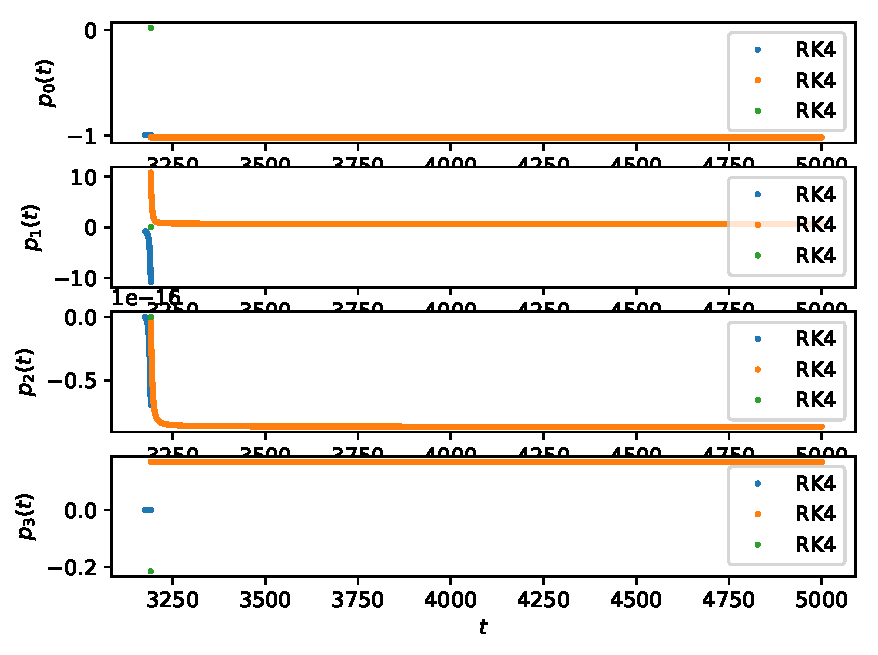
\includegraphics[height=8cm]{Figures/U_t_Penrose.pdf}
	\caption[Run 3: 4-momentum]{Run 3: 4-momentum for the simulated Penrose process.}
	\label{fig:RUN3_U}
\end{figure}
\section{Comments and Discussion}
\label{Sec4}

\subsection{Part A: Solving Geodesics}
As is obvious, the trajectories simulated are in agreement with the expected observations. For the first run, the trajectory is bounded and the energy ($E = -mu_{0}$) and angular momentum ($L = mu_{3}$) are conserved. The conservation laws also hold in the second in-falling trajectory but some expected instabilities seem to add up as the particle approaches more and more the event horizon at $r=2.0$. This just a computational artifact coming from the singular behavior of the metric at the event horizon. What is remarkable is that the particle slows down as it approaches the event horizon until it eventually stop at $r=2.0$; this is the expected behavior as seen by a stationary observer.

\subsection{Part B: Simulating the Penrose Process}
The results speak for themselves. Particle 3 does indeed have a negative energy, while particle 2 has sufficient energy to escape to infinity ($\epsilon_2>1$). The final terminal velocity will have only a radial non-zero component with value\footnote{Since energy is conserved, we simply set the asymptotic behavior of the metric $g_{\mu\nu} \rightarrow \eta_{\mu\nu}$,
\be
	\epsilon = u_{0} \rightarrow \frac{1}{\sqrt{1-\upsilon_{r\infty}}}
\ee },
\be
	v_{2\infty} = \sqrt{1-\frac{1}{\epsilon_2^2}} = 0.687015393
\ee

The efficiency of the particular process is,
\be
	\eta = \frac{E_2}{E_1} = \mu_2\frac{\epsilon_2}{\epsilon_1} = 102.15 \%
\ee
In other words, particle 2 has gained $2.15 \%$ more energy than the initial parent particle!
\section{Perspectives}
\label{Sec5}

The analysis demonstrated has been successful to simulate the Penrose process. Further applications would be to investigate more into the limits of the process in terms of its efficiency. An even more interesting extension would be to add a non-zero electrical charge on the particles. Then, there will be an additional Lorentz force that actually favors the Penrose process (\cite{PenroseProcessCharged}). Simulation of this generalized Penrose process could shine more light on the natural mechanisms allowing a physical black hole to appear energetic to a distant observer.

Eventually, we would like to also simulate the Blandford-Znajek process (\cite{Blandford1977}) which is believed to be the main mechanism explaining the incredible power emitted by quasars but for now, we submit the process so far.
\begin{appendices}
	\noappendicestocpagenum
	\section{Derivation of equations of motion}
\label{ApA}

In this appendix, we derive the equations of motion \eqref{EOM_F} for a massive particle. To derive them, we start from the geodesics equations,
\be
	\ddot{x} + \Gamma^{\rho}_{\mu\nu}\dot{x}^{\mu}\dot{x}^{\nu} = a^{\rho}
\ee
and write all the derivatives with respect to the proper time $\tau$ in term of derivatives with respect to the coordinate time $t$. For the $D$-velocity, we have,
\be
	\dot{x}^{\mu} = \dot{t}\upsilon^{\mu}
\ee
while, for the $D$-acceleration, we have,
\be\ba
	\ddot{x}^{\mu} &= \left(\dot{x}^{\mu}\right)\dot{} \\
	&= \ddot{t}\upsilon^{\mu} + \dot{t}^2\frac{d\upsilon^{\mu}}{dt} \\
	&= \dot{t}^2\left(\frac{d\upsilon^{\mu}}{dt} - \Gamma^{0}_{\mu\nu}\upsilon^{\mu}\upsilon^{\nu}\right) + a^{0}\upsilon^{\mu}
\ea\ee
where we used the $0$-component of the geodesics in the third line. Lastly, we use the normalization of the $D$-velocity for massive particles to express $\dot{t}$ in terms of the coordinate velocity,
\be\ba
	u_{\mu}u^{\mu} &= g_{\mu\nu}u^{\mu}u^{\nu} = \dot{t}^2g_{\mu\nu}\upsilon^{\mu}\upsilon^{\nu} = -1 \\
	&\Rightarrow \dot{t} = \frac{1}{\sqrt{-g_{\mu\nu}\upsilon^{\mu}\upsilon^{\nu}}}
\ea\ee
and plug everything back to the geodesics to extract the equations of motion for the coordinate velocity,
\be\ba
	\frac{d\upsilon^{\rho}}{dt} &= \left(\Gamma^{0}_{\mu\nu}\upsilon^{\rho}-\Gamma^{\rho}_{\mu\nu}\right)\upsilon^{\mu}\upsilon^{\nu} + \frac{a^{\rho} - a^{0}}{\dot{t}^2} \\
	&= \left(\Gamma^{0}_{\mu\nu}\upsilon^{\rho}-\Gamma^{\rho}_{\mu\nu} - g_{\mu\nu}(a^{\rho} - a^{0})\right)\upsilon^{\mu}\upsilon^{\nu} 
\ea\ee
	\section{Coordinate velocitiy Vs $D$-velocity}
\label{ApB}

In this small appendix, we analyze the equivalence of giving the coordinate velocity components $\upsilon^{\mu}=(1,\vec{\upsilon})$ and giving the covariant\footnote{We consider the covariant $D$-velocity because it includes the usual conserved charges. For example, the energy is defined by $E=-mu_{0}$ and the angular momentum associated with rotations around the $x_{d}$-axes is given by $L=mu_{d}$ when using spherical coordinates.} $D$-velocity $u_{\mu}$. Although there are only $D-1$ independent components for the coordinate velocity, there is the additional parameter of the rest mass $m$ of the massive particle resulting in an equal number of spatial components of the coordinate velocity $\vec{\upsilon}$ and independent components of the $D$-velocity $u_{\mu}$. The rest mass can be immediately obtained from,
\be
	p^2 = -m^2
\ee
from which the condition $u^2 = -1$ for massive particles follows. The notation of the norm of a $D$-vector $A^{\mu}$ here is,
\be
	A^2 \equiv A_{\mu}A^{\mu} = g_{\mu\nu}A^{\mu}A^{\nu}
\ee
As a result we can determine the coordinate velocity $\vec{\upsilon}$ from $D-1$ components of the of the $D$-velocity $u_{\mu}$. To simplify things to situations that are very common, we assume that we know all the vectorial components of the coordinate velocity apart from the $i$'th component, that is, we know $\upsilon^{l}$, $l=1,\dots,i-1,i+1,\dots,D-1$ but not $\upsilon^{i}$. Then, given, one of the components of the $D$-velocity, say the $\mu$'th component, it can be shown that $\upsilon^{i}$ is given by,
\be\ba
	\upsilon^{i} &= \frac{-\beta_{i\mu} \pm \sqrt{\beta_{i\mu}^2 - \alpha_{i\mu}\gamma_{i\mu}}}{\alpha_{i\mu}} \\
	\alpha_{i\mu} &= u_{\mu}^2 g_{ii} + g_{\mu i}^2 \\
	\beta_{i\mu} &= u_{\mu}^2 \left(g_{0i} + g_{il}\upsilon^{l}\right) + g_{\mu i}\left(g_{\mu0} + g_{\mu l}\upsilon^{l}\right) \\
	\gamma_{i\mu} &= u_{\mu}^2 \left(g_{00} + 2g_{0l}\upsilon^{l} + g_{lm} \upsilon^{m}\upsilon^{l}\right) + \left(g_{\mu0} + g_{\mu l}\upsilon^{l}\right)^2
\ea\ee
where there is no sum over the $mu$ and $i$ indices, while the summation over $m$ and $l$ runs from $1$ to $D-1$ excluding the value $i$. To decide the ``$+$'' or ``$-$'' sign, one just plugs $\upsilon^{i}$ in the expression for $u_{\mu}$ and checks which sign gives the right answer.

For more practical applications of this procedure, we take the $\mu=i$. In this case, the results simplify and become,
\be\ba\label{vi_ui}
	\upsilon^{i} &= -\frac{g_{0i} + g_{il}\upsilon^{l}}{g_{ii}} + u_{i} \sqrt{\Delta_{i}} \\
	\Delta_{i} &= \frac{\left(g_{0i} + g_{il}\upsilon^{l}\right)^2 - g_{ii}\left(g_{00} + 2g_{0l}\upsilon^{l} + g_{lm} \upsilon^{m}\upsilon^{l}\right)}{g_{ii}^2 \left( u_{i}^2 + g_{ii} \right) }
\ea\ee
This prescription will prove useful for determining the initial conditions for the Penrose process to be observed.

	\section{$D$-momentum Vs Conjugate momenta}
\label{ApC}

Here, we emphasize on the difference between the $D$-momentum $p_{\mu}$ appearing in General Relativity versus the conjugate momenta of a particle system described by a Lagrangian $L$. The $D$-momentum components for a massive particle are defined by,
\be
	p_{\mu} = mu_{\mu}
\ee
with $u_{\mu}$ the covariant $D$-velocity components. In terms of the coordinate velocity components, $p_{\mu}$ are written as,
\be
	p_{\mu} = m\frac{g_{\mu\nu}\upsilon^{\nu}}{\sqrt{-g_{\rho\sigma}\upsilon^{\rho}\upsilon^{\sigma}}} = m\frac{g_{\mu0}+g_{\mu i}\upsilon^{i}}{\sqrt{-\left(g_{00} + 2g_{0j}\upsilon^{i} + g_{jk}\upsilon^{j}\upsilon^{k}\right)}}
\ee
In the absence of any non-gravitational interactions, the $D$-momentum components are also the conjugate momenta,
\be
	P^{\mu} = \frac{\partial \mathcal{L}}{\partial u_{\mu}}
\ee
with $\mathcal{L}$ the Lagrangian describing the system. The gravitational part reads,
\be
	\mathcal{L}_{gr} = \frac{1}{2}mu^2 = \frac{1}{2}mg_{\mu\nu}u^{\mu}u^{\nu}
\ee
where we have adopted the notation for the norm of a $D$-vector $A^{\mu}$,
\be
	A^2 \equiv A_{\mu}A^{\mu} = g_{\mu\nu}A^{\mu}A^{\nu} = g^{\mu\nu}A_{\mu}A_{\nu}
\ee

If the Lagrangian contains additive new terms $\mathcal{L}_{int}$ associated with non-gravitational interactions, e.g. electromagnetic interactions,
\be
	\mathcal{L} = \mathcal{L}_{gr} + \mathcal{L}_{int}
\ee
then the conjugate momenta are,
\be
	P_{\mu} = p_{\mu} + \frac{\partial \mathcal{L}_{int}}{\partial u^{\mu}}
\ee
The conjugate momenta are useful observables from which ordinary constants of motion can be read from. For example, the energy is defined by $E \equiv -P_{0}$.

The Euler-Lagrange equations then become the geodesics in the presence of non-gravitational forces,
\be
	\dot{u}^{\rho} + \Gamma^{\rho}_{\mu\nu}u^{\mu}u^{\nu} = a^{\rho}
\ee
with the non-gravitational $D$-acceleration $a^{\rho}$ constructed entirely from the interaction Lagrangian,
\be\ba
	a^{\rho} &= \frac{g^{\rho\mu}}{m}\left( \partial_{\mu} \mathcal{L}_{int} - \frac{d}{d\tau}\left( \frac{\partial \mathcal{L}_{int}}{\partial u^{\mu}} \right) \right) \\
	&= \frac{g^{\rho\mu}}{m}\left( \partial_{\mu} \mathcal{L}_{int} - u^{\nu}\partial_{\nu}\left( \frac{\partial \mathcal{L}_{int}}{\partial u^{\mu}} \right) - \dot{u}^{\nu}\frac{\partial \mathcal{L}_{int}}{\partial u^{\mu}\partial u^{\nu}} \right)
\ea\ee
In the above expansion of the $D$-acceleration we made the very natural assumption that the interaction Lagrangian only depends on the spacetime position $x^{\mu}$ and the $D$-velocity $u^{\mu}$.

\subsection{Example: Lorentz force}
If the background metric describes an electrically charged mass distribution, e.g. a charged black hole, then a massive particle that also carries an electric charge $q$ will also experience a Lorentz force. This is inputted in the Lagrangian by the term,
\be
	\mathcal{L}_{int} = qA_{\mu}u^{\mu}
\ee
with $A_{\mu}$ the $x^{\mu}$-dependent covariant $D$-potential created by the charged mass configuration. We assume here that the background electromagnetic field created is stationary. Then the $D$-acceleration is,
\be
	a^{\rho} = \frac{q}{m}F^{\rho}_{\;\;\sigma}u^{\sigma}
\ee
with $F_{\mu\nu}$ the electromagnetic field strength tensor\footnote{The operation of anti-symmetrization of a rank-2 tensor $T_{\mu\nu}$ is,
\be
	T_{[\mu\nu]} \equiv \frac{1}{2}\left( T_{\mu\nu} - T_{\nu\mu} \right)
\ee},
\be
	F_{\mu\nu} = 2\nabla_{[\mu}A_{\nu]} = 2\partial_{[\mu}A_{\nu]}
\ee
while the conjugate momenta read,
\be
	P_{\mu} = p_{\mu} + qA_{\mu}
\ee
\end{appendices}

\addcontentsline{toc}{section}{References}
\bibliographystyle{plain}
\bibliography{FinalProject_References}
\end{document}